\chapter{\label{chap:modeling}Modelagem do Sistema}

Conforme visto na subseção \ref{subsec:simulation:components}, um sistema de
simulação possui uma série de componentes conceituais, cada um tendo suas
responsabilidades bem definidas. Para o projeto do simulador de sistemas de
elevadores deste estudo, doravante chamado apenas de simulador, optou-se pelo
paradigma de Programação Orientada à Objetos. Esta opção se deu pelos seguintes
motivos:

\begin{description}
  \item[Elevada Capacidade de Abstração]\hfill \\
    Conceitos da Programação Orientada à Objetos, como classes, interfaces,
    polimorfismo, herança e sobrecarga permitem a realização de uma modelagem
    conceitual em alto nível de abstração, permitindo uma explanação de fácil
    entendimento sem ser necessário abordar questões da implementação em si
    (linguagem de programação, arquitetura, etc).
  \item[Padrão de Mercado]\hfill \\
    Desde meados dos anos 90, a Programação Orientada à Objetos tornou-se o mais
    frequentemente utilizado no mercado de desenvolvimento de software e nos
    ambientes acadêmicos relacionados à computação. Assim, é possível atingir
    uma maior audiência.
  \item[Domínio dos Autores]\hfill \\
    O paradigma é de domínio dos autores deste estudo.
\end{description}

Nas próximas seções serão apresentadas as construções para o projeto do
simulador de elevadores.

\section{Eventos e Tipos}

A simulação de eventos discretos, como o próprio nome já diz, é totalmente
orientada à eventos. Isso significa dizer que as alterações no estado do sistema
ocorrerão somente na ocasião de algum evento. Sendo assim, é necessária uma
representação de um evento no projeto do simulador.

Um evento é uma estrutura que deve possuir as seguintes informações: (1) o tipo
do evento; (2) o horário agendado para a ocorrência do evento; (3) um cliente
(passageiro) e/ou (4) um elevador e/ou (5) um andar do prédio. As existência de
informações para os itens (3), (4) e (5) dependem do tipo de evento, que pode
ser uma das seguintes opções:

\begin{description}
  \item[Chegada de um cliente] \hfill \ um cliente chegou na fila de um andar
  \item[Chegada de um elevador] \hfill \ um elevador chegou a um andar e abriu as portas
\end{description}

Para o evento \textbf{chegada de um cliente}, é necessário conhecer o cliente e
o andar. Para o evento \textbf{chegada de um elevator}, é necessário conhecer o
elevador e o andar. A figura \ref{fig:diagram:event} exibe o diagrama de classes
para eventos e tipos de evento. Adicionalmente foi criada a classe
\textit{Config}, que irá armazenar as informações do cenário de testes.

\begin{figure}[htb!]
  \centering
  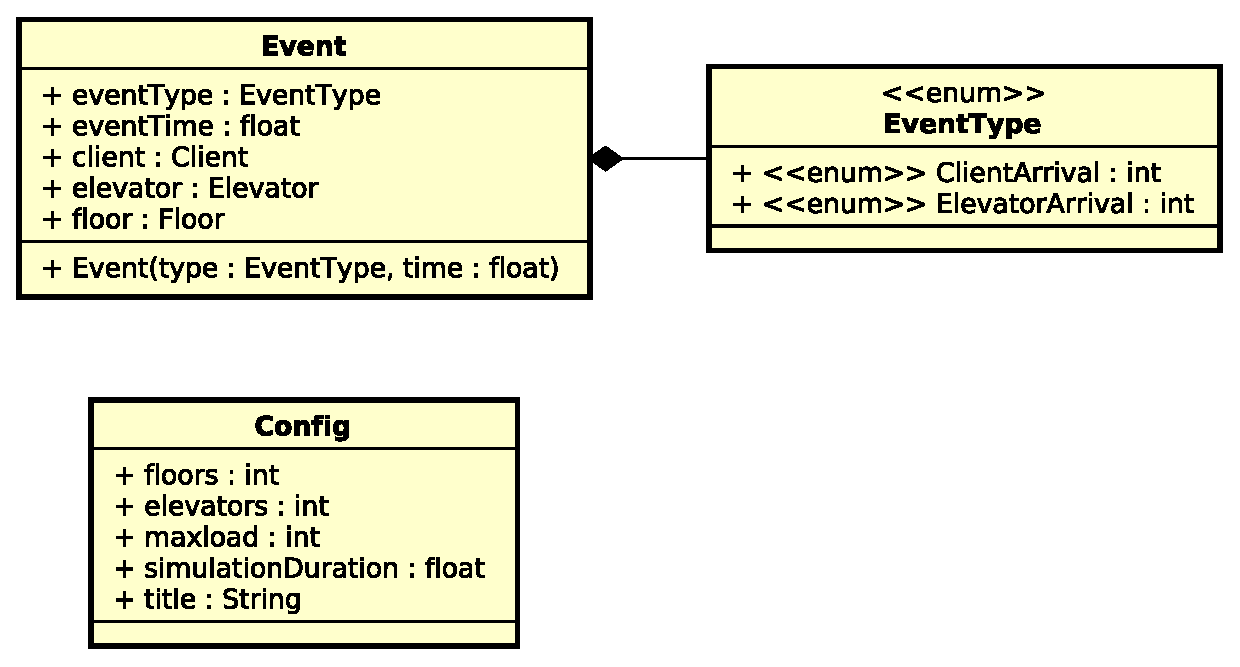
\includegraphics[scale=0.6]{img/Basic.eps}
  \caption{Diagrama de classes para eventos, tipos de eventos e configuração da simulação.}
\label{fig:diagram:event}
\end{figure}

\section{\label{sec:model:notify}Notificando Eventos: o padrão
\textit{Observer}}

Em um simulador, há a necessidade de executar diferentes ações na ocasião de um
evento específico - cada tipo de evento possui uma \textit{Rotina de Evento}
correspondente, responsável por atualizar o estado do sistema, as estatísticas e
o relógio da simulação. Em termos genéricos, quando ocorrer uma alteração em um
objeto~-~um evento ocorreu~-,~outros objetos devem ter o seu estado alterado em
função disso. De acordo com Gamma \cite{Gamma:1995:DPE:186897}, o padrão
\textit{Observer} é um \textit{design pattern} indicado para resolver este
problema. Este \textit{pattern} define uma dependência de um-para-muitos ($1:N$)
entre objetos de modo que, quando este um objeto (\textit{subject}) tem seu
estado alterado, todos os seus dependentes (\textit{observers}) são notificados
deste mudança. Por consequência, estes dependentes podem modificar seu estado
interno baseando-se nas informações desta notificação. Neste projeto, o
subsistema que segue o \textit{Observer pattern} será chamado de \textit{SNE},
acrônimo para \textit{Sistema de Notificação de Eventos}.

Os três principais componentes do \textit{SNE} (figura
\ref{fig:diagram:notification}) são duas interfaces e uma classe:

\begin{description}
  \item[EventObserver] \hfill \\
    Interface a ser realizada por qualquer classe que deseje receber
    notificações de eventos. Seu único método, \texttt{notify}, permite o
    recebimento de uma notificação de um evento.

  \item[EventNotifier] \hfill \\
    Interface a ser realizada por qualquer classe que deseje notificar a
    ocorrência de eventos. Define métodos que objetos que implementem a
    interface \textit{EventObserver} possam se registrar (\texttt{register}) ou
    desregistrar (\texttt{unregister}) para receber notificações de ocorrências
    de um determinado tipo de evento, além do método \texttt{notify}, que deverá
    notificar um evento para todos os \textit{observers} registrados.

\item[EventDispatcher] \hfill \\
    Classe concreta que realiza a interface \textit{EventNotifier}. Deve possuir
    uma estrutura de dados para armazenar quais \textit{observers} se
    registraram para cada tipo de evento. Na ocorrência de um evento, o
    \textit{EventDispatcher} é responsável por varrer a lista de
    \textit{observers} registrados e notificá-los de acordo com o tipo de evento
    ocorrido.

\end{description}

\begin{figure}[htb!]
  \centering
  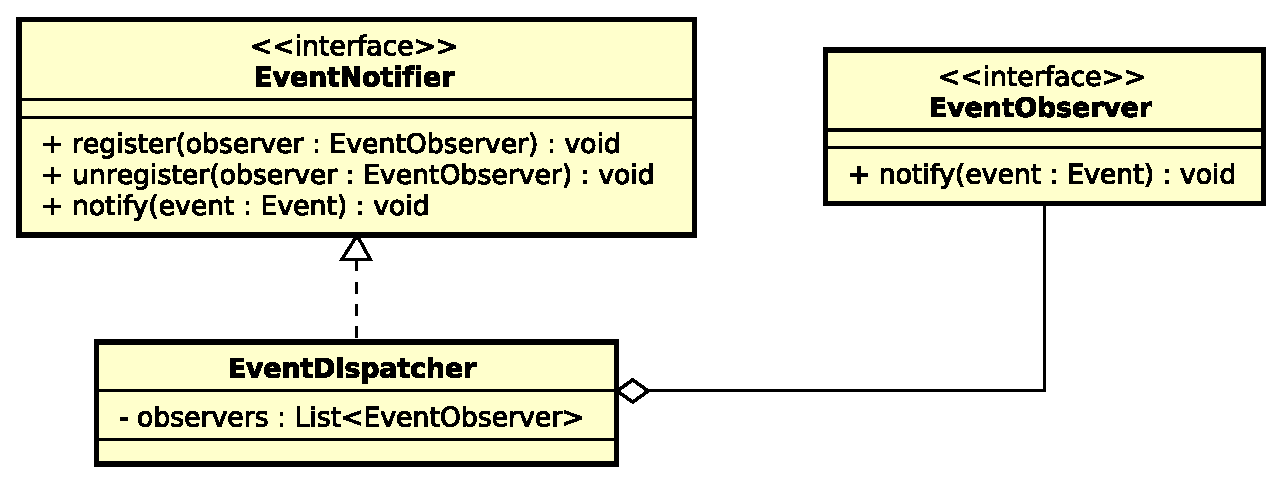
\includegraphics[scale=0.6]{img/Notification.eps}
  \caption{Diagrama de classes do \textit{Sistema de Notificação de Eventos}.}
\label{fig:diagram:notification}
\end{figure}

Três importantes componentes do simulador podem se beneficiar desta construção:
(1) o \textit{relógio do sistema} (classe \textit{Timer}); (2) os
\textit{contadores estatísticos} (classe \textit{Statistics}); e (3) o
\textit{estado do sistema} (classe \textit{Building}). Na ocorrência de um
evento, estas três entidades devem ser notificadas e cada uma irá alterar seu
estado interno da forma que lhe convir. Para isto, devem implementar a interface
\textit{EventObserver} e registrarem-se no \textit{EventDispatcher}, conforme
ilustrado na figura \ref{fig:diagram:observers}.

\begin{figure}[htb!]
  \centering
  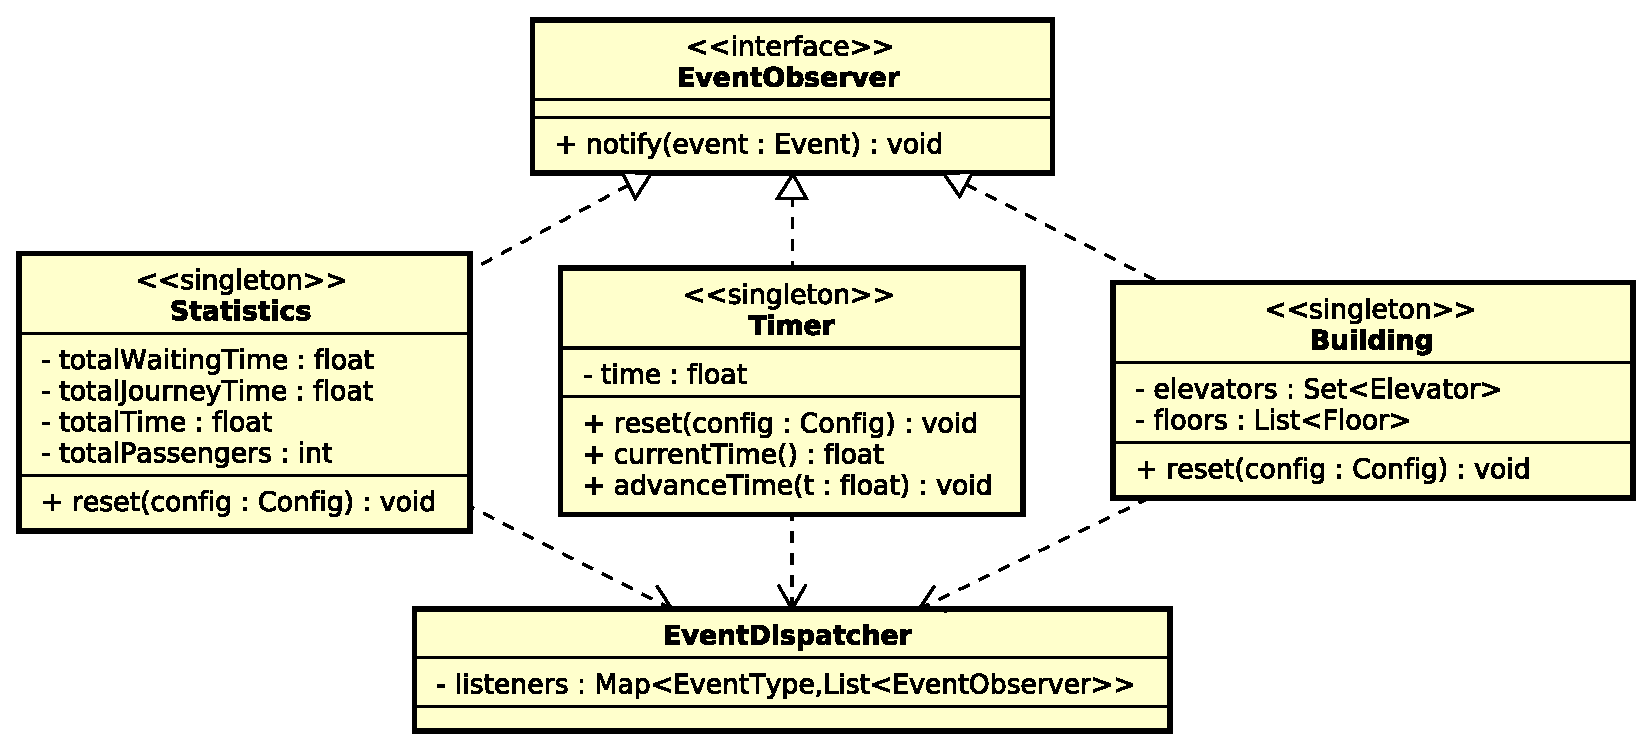
\includegraphics[scale=0.6]{img/Observers.eps}
  \caption{Diagrama de classes dos \textit{observers}.}
\label{fig:diagram:observers}
\end{figure}

\section{Gerenciamento de Eventos com Prioridades}

Conforme visto na seção \ref{sec:model:notify}, o \textit{EventDispatcher} é
responsável por notificar as partes interessadas da ocorrência de um evento.
Porém não responde a questão de qual deve ser o próximo evento que irá ocorrer.

Na seção \ref{chap:sim:timeadvance} foi apresentado o \textit{mecanismo de
avanço de tempo para o próximo evento}, onde deve-se verificar, em uma lista de
eventos, qual é o próximo evento a ocorrer. Dado um conjunto de eventos
agendados (ou seja, ainda não ocorridos), o primeiro evento a ocorrer é
justamente o que possui o menor tempo de agendamento. Um tipo abstrato de dados
que serve para este propósito é uma \textit{fila prioritária}, ou
\textit{priority queue}. Uma \textit{fila prioritária} funciona de forma similar
a filas \textit{FIFO}, com a diferença de que cada elemento armazenado possui
uma prioridade associada. A \textit{fila prioritária} irá atender os elementos
por ordem de prioridade, da maior para a menor. Ao considerar que a prioridade
de um evento é inversamente proporcional ao instante em que irá ocorrer - ou
seja, quanto menor o tempo do evento maior é a sua prioridade -, temos uma fila
na qual o próximo elemento a ser atendido sempre será o próximo evento a
ocorrer.

Assim, a classe \textit{EventQueue} encapsula uma fila prioritária de eventos,
fornecendo métodos para inserir um evento na fila (\texttt{push}), recuperar e
remover o próximo evento (\texttt{pop}) ou simplesmente ``espiar'' o próximo
evento (\texttt{peek}). Juntamente com a classe
\textit{EventGenerator}\footnote{Classe responsável pela criação de eventos;
abordada mais adiante neste estudo.}, a \textit{EventQueue} compõe o chamado
\textit{Sistema de Gerência de Eventos}, ou \textit{SGE}. Assim, possibilita-se
que o \textit{EventDispatcher} facilmente recupere próximo evento a ocorrer e
dispare as notificações.

\begin{figure}[htb!]
  \centering
  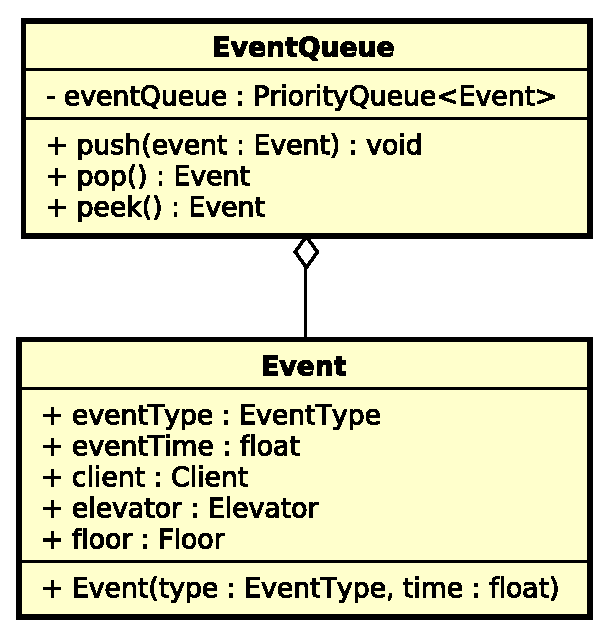
\includegraphics[scale=0.6]{img/EventQueue.eps}
  \caption{Diagrama de classes do \textit{Sistema de Gerência de Eventos}.}
\label{fig:diagram:event:manage}
\end{figure}

\section{Estado do Sistema: o Prédio e suas Partes}

A seção \ref{sec:model:notify} apresentou o conceito de \textit{observers}.
Dentre os listados, encontra-se a classe \textit{Building}. Esta classe é
responsável por encapsular o \textit{Estado do Sistema} (figura
\ref{fig:diagram:system}), gerenciando instâncias de elevadores
(\textit{Elevator}), andares (\textit{Floor}) e clientes (\textit{Client}).

\begin{figure}[htb!]
  \centering
  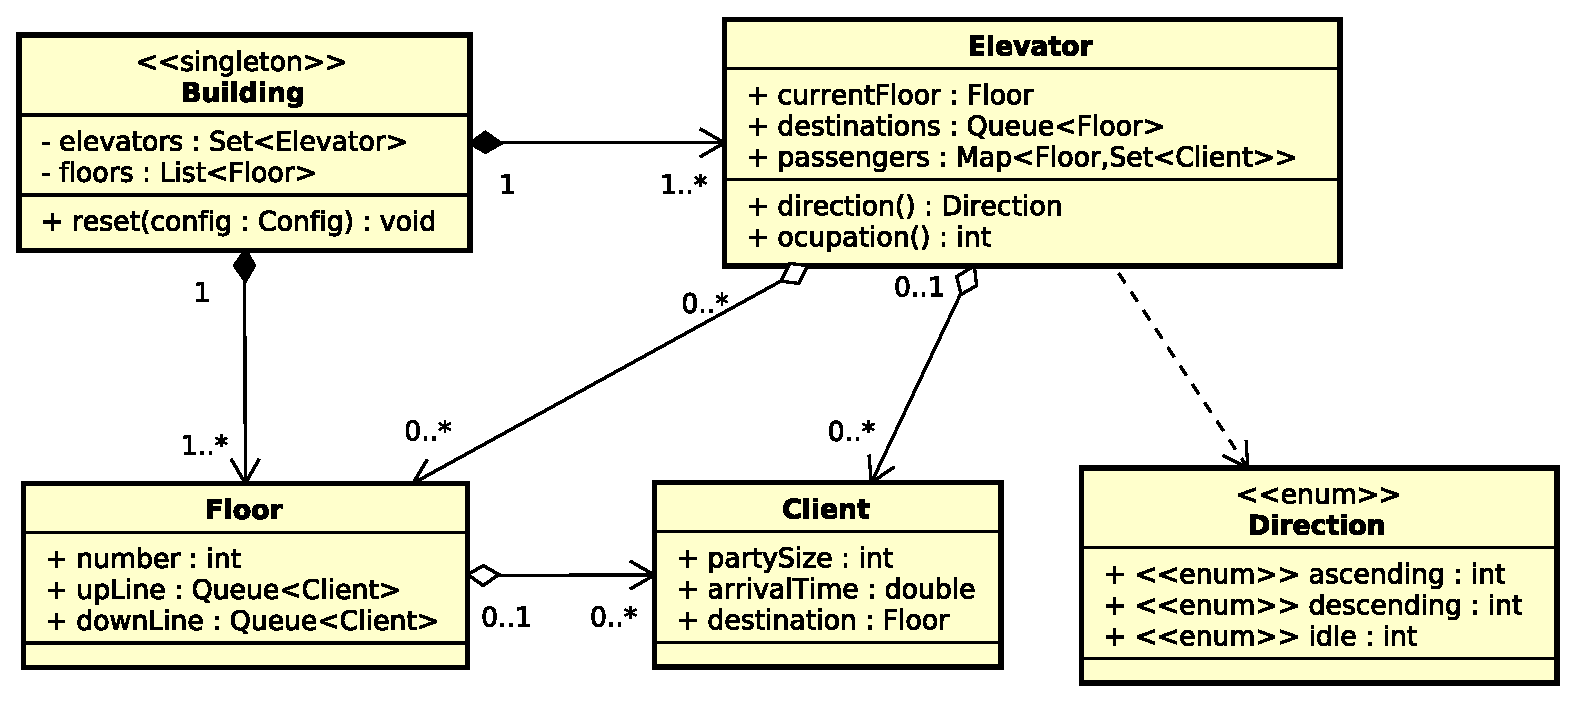
\includegraphics[scale=0.6]{img/Model.eps}
  \caption{Diagrama de classes do \textit{Estado do Sistema}.}
\label{fig:diagram:system}
\end{figure}

\begin{description}
  \item[Building] \hfill \\
    Representa a composição o prédio sendo simulado. Possui um conjunto de
    elevadores, uma lista ordenada de andares e um método \texttt{reset},
    utilizado para a inicialização da simulação. Um prédio é formado por no
    mínimo um elevador e no mínimo um andar\footnote{Isto em termos conceituais;
    porém, não há sentido na existência de um sistema de elevadores em uma
    edificação com somente um andar. De fato, conforme afirmado na seção
    \ref{section:scenarios}, serão simulados prédios com, no mínimo, 4
    andares.}.

  \item[Floor] \hfill \\
    Parte componente de um prédio, possuindo uma numeração e duas
    filas\footnote{No mundo real, apesar de aparentemente as pessoas formarem
    uma fila única, os membros da fila respeitam o sentido de viagem do elevador
    e implicitamente separam-se em duas filas: uma para subir e outra para
    descer.}: uma para clientes que desejam descer e outra para clientes que
    desejam subir.

\item[Elevator] \hfill \\
    Representa um elevador único. Possui como atributos o andar em que se
    encontra, uma sequência ordenada de andares destinos, e um mapa associando
    andares com conjuntos de clientes - ou seja, agrupa, para cada andar, quais
    os grupos de clientes que o possuem como destino. Além disso, possui métodos
    auxiliares para informar o sentido da viagem do elevador
    (\texttt{direction}), bem como a sua ocupação atual (\texttt{ocupation}).

\item[Client] \hfill \\
    Representa um grupo de pessoas que desejam utilizar um elevador. Possui como
    atributos o tamanho do grupo, o horário em que chegou na fila do andar e o
    andar destino para o qual deseja ir.

\end{description}

\section{Simulador}

O componente responsável por orquestrar todas as interações entre as classes
descritas nas seções anteriores é representado pela classe \textit{Simulator}.

\begin{figure}[htb!]
  \centering
  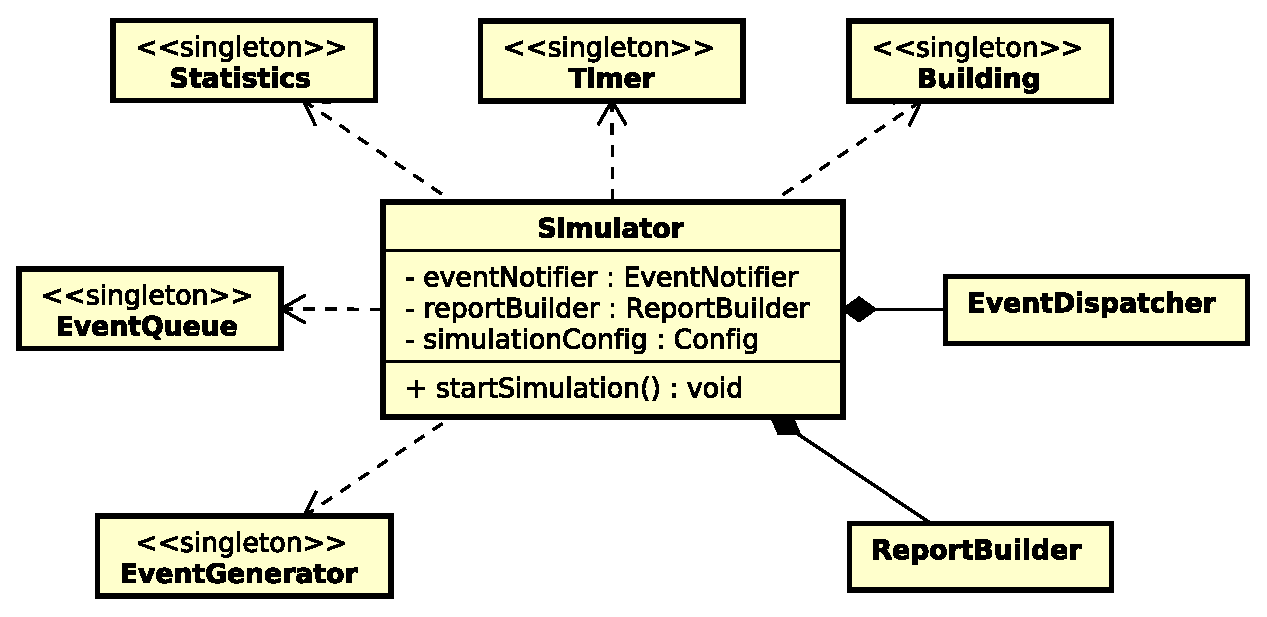
\includegraphics[scale=0.6]{img/Simulator.eps}
  \caption{Diagrama de Classes do Simulador}
\label{fig:diagram:simulator}
\end{figure}

\begin{algorithm}[htb]
\begin{center}
\begin{algorithmic}[1]
\Function{doSimulation}{$timer, statistics, building, eventQueue, eventDispatcher, reportBuilder$}
  \State $timer.$\Call{reset}{ }
  \State $statistics.$\Call{reset}{ }
  \State $building.$\Call{reset}{ }
  \State $eventDispatcher.$\Call{register}{$EventType.Any, timer$}
  \State $eventDispatcher.$\Call{register}{$EventType.Any, building$}
  \State $eventDispatcher.$\Call{register}{$EventType.Any, statistics$}
  \While{\Call{MustSimulationRun}{ } = $true$}
    \State $nextEvent \leftarrow eventQueue.$\Call{pop}{\ }
    \State $eventDispatcher.$\Call{notify}{$nextEvent$}
  \EndWhile
  \State $reportBuilder.$\Call{buildReport}{$config, statistics$}
\EndFunction
\end{algorithmic}
\end{center}
\caption
   {\label{alg:base}Algoritmo Base}
\end{algorithm}

\section{\label{sec:model:report}Gerando Relatórios}

Por último, porém não menos importante, é apresentado o \textit{Sistema de
Geração de Relatórios}, ilustrado pela figura \ref{fig:diagram:report}. Este
sistema nada mais é do que um componente que recebe a configuração da simulação
e os dados estatísticos coletados e monta relatórios sintéticos e anaĺiticos com
informações relevantes.

\begin{figure}[htb!]
  \centering
  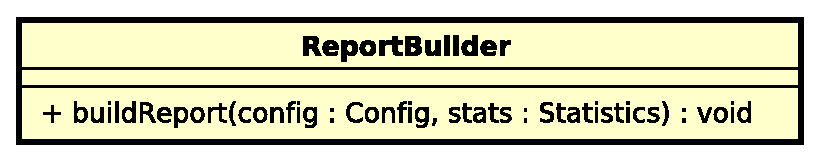
\includegraphics[scale=0.6]{img/Report.eps}
  \caption{Diagrama de classes do \textit{Sistema de Geração de Relatórios}.}
\label{fig:diagram:report}
\end{figure}

\section{\label{sec:model:generator}Criação de Eventos}

\begin{figure}[htb!]
  \centering
  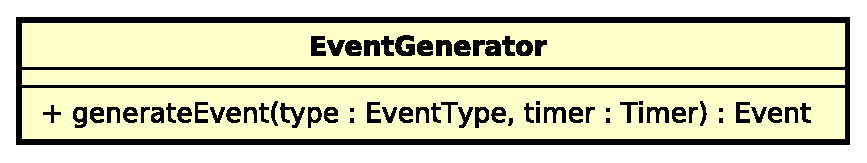
\includegraphics[scale=0.6]{img/EventGenerator.eps}
  \caption{Diagrama de classes do \textit{Sistema de Geração de Eventos}.}
\label{fig:diagram:generator}
\end{figure}

\section{\label{chap:input}Entrada de Distribuição de Probabilidade}

Aqui vamos apresentar:

\begin{itemize}
\item Conceitos sobre distribuições de probabilidade;
\item Conceitos sobre geração de variáveis aleatórias em ambiente computacional;
\item Descrever o modelo selecionado de processo de chegada de clientes
(passageiros);
\item Algoritmos e fluxogramas dos eventos do simulador que causarão alterações
no estado do sistema.
\end{itemize}